\section{Results}
\label{sec:results}

\subsection{Tuning Learning Rate and Minibatch Size}

\subsubsection*{Logistic Regression}
Figure \ref{fig:TuneLogReg_auc} shows a heatmap of the AUC of the Logistic Regression model used on the classification problem for different minibatch sizes and initial learning rates, where the variables are distributed logarithmically. The blank fields represents variables that gave overflow. 
\begin{figure}[htbp]
	\centering
	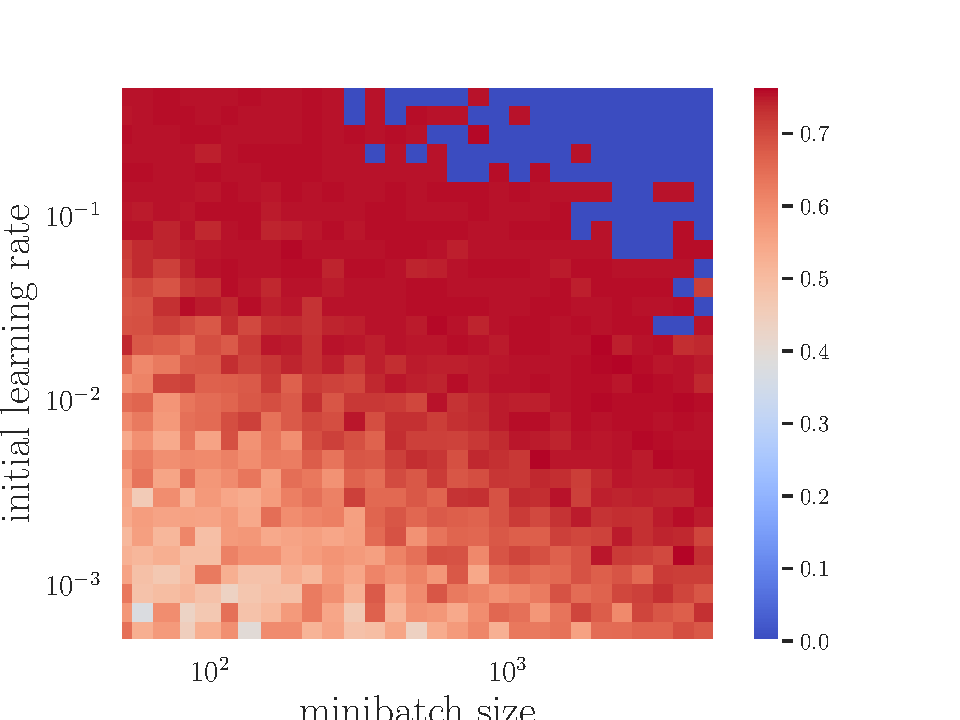
\includegraphics[width=0.5\textwidth]{LogRegTune_auc}
	\caption{Heatmap showing the AUC of the Logistic Regression for different
		values of the minibatch sizes and initial learning rates.}
	\label{fig:TuneLogReg_auc}
\end{figure}

Figure \ref{fig:TuneLogReg_accuracy} is similar to Figure \ref{fig:TuneLogReg_auc}, except that the heatmap shows the accuracy, and not the AUC, for the Logistic Regression. 
\begin{figure}[htbp]
	\centering
	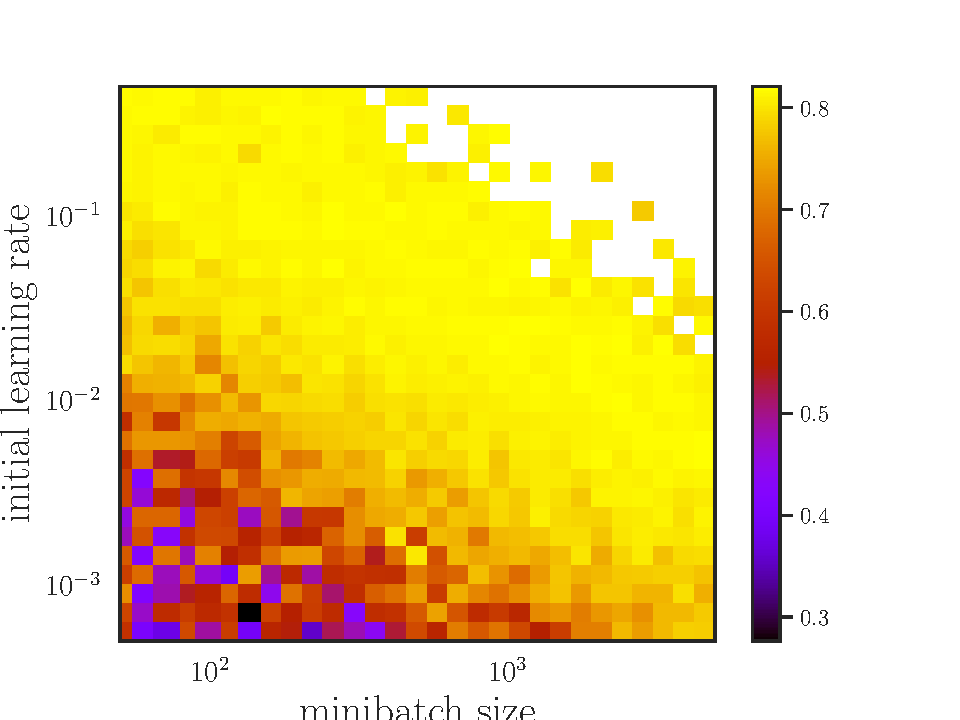
\includegraphics[width=0.5\textwidth]{LogRegTune_accuracy}
	\caption{Heatmap showing the accuracy of the Logistic Regression for different values of the minibatch sizes and initial learning rates.}
	\label{fig:TuneLogReg_accuracy}
\end{figure}

\subsubsection*{Neural network}
\begin{figure}[htbp]
	\centering
	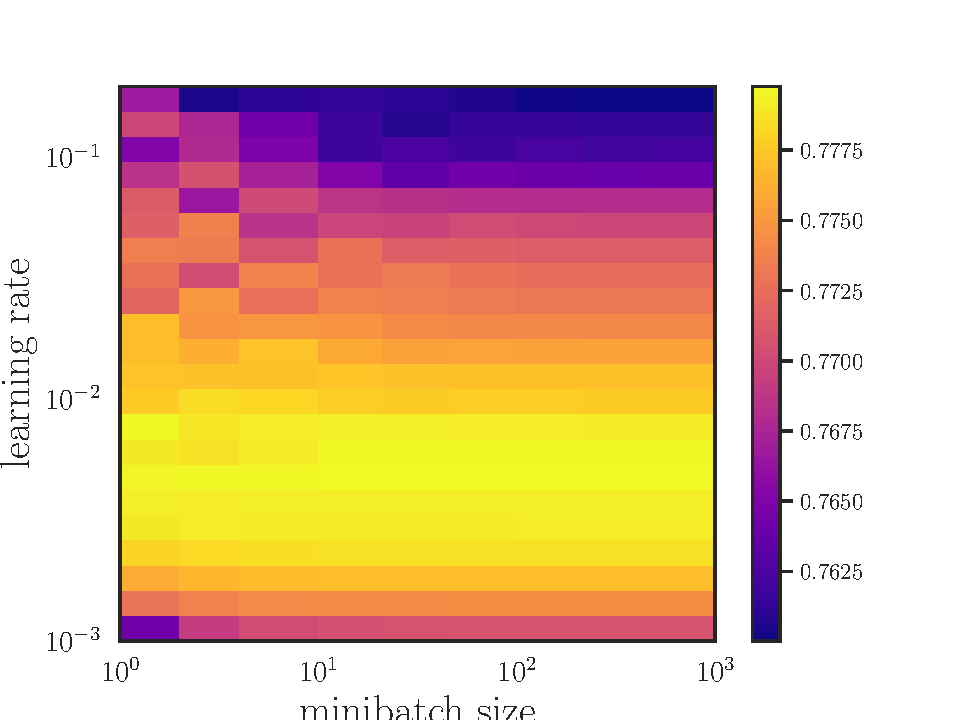
\includegraphics[width=0.5\textwidth]{NNTune_auc}
	\caption{Heatmap showing the AUC of the Neural Network for different
		values of the minibatch sizes and learning rates.}
	\label{fig:TuneNN_auc}
\end{figure}

\begin{figure}[htbp]
	\centering
	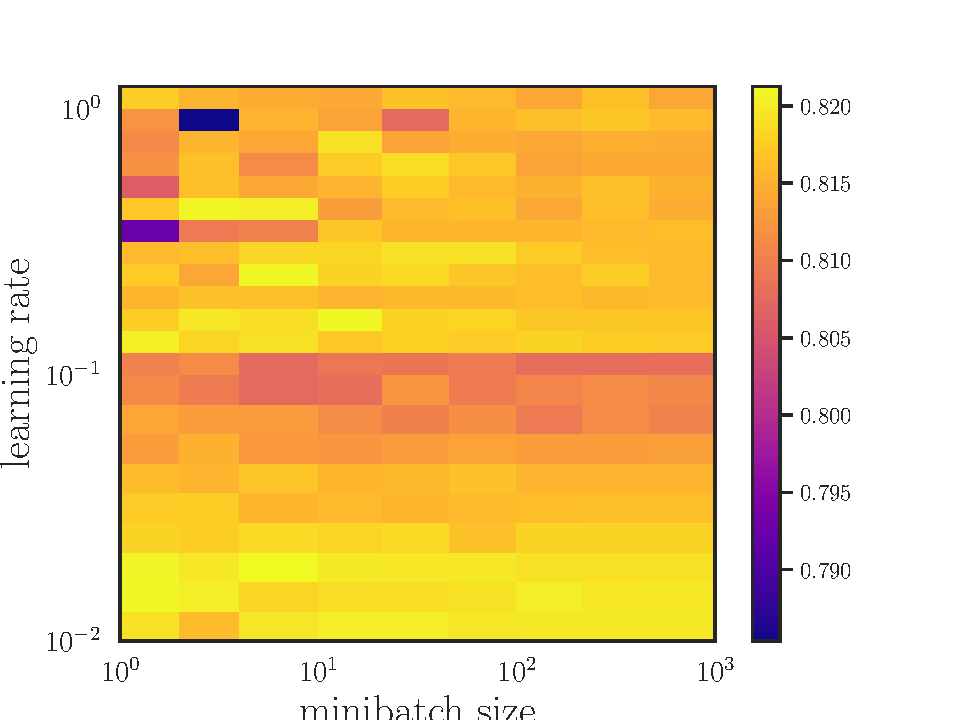
\includegraphics[width=0.5\textwidth]{NNTune_accuracy}
	\caption{Heatmap showing the accuracy of the Neural Network for different
		values of the minibatch sizes and learning rates.}
	\label{fig:TuneNN_accuracy}
\end{figure}

\subsection*{Optimal Parameters and Associated Results}

\subsection{Verification by Comparison to Scikit-Learn}

\subsection{Neural Networks for Regression on Franke's Function}


% Eksempel for figurer
\begin{table}[htbp]
\renewcommand{\arraystretch}{1.2}
\caption{Fraction of true and false negatives and positives for Logistic regression, Neural network, and SciKit Learn applied on the classification problem.}
	\begin{tabular}{p{18mm} l l l l}
		\toprule
		Method & \multicolumn{2}{l}{Positive} & \multicolumn{2}{l}{Negative} \\
		\cline{2-3} \cline{4-5}
		& True & False & True & False \\
		\midrule
		Logistic \newline regression & 0.67 & 0.33 & 0.84 & 0.16 \\
		Neural \newline network & TBA & TBA & TBA & TBA \\
		\bottomrule
	\end{tabular}
\label{tab:confusion}
\end{table}


